\documentclass{amsart}

\input{../preamble_general.tex}

\author{Jalen Chrysos}
\title{More About Planar Graphs (with Solutions)}

\begin{document}
	\maketitle 
	
	\noindent \textbf{Problem}: 
	\begin{enumerate}[(a)]
		\item Suppose we want to make a soccer ball using \textit{only} hexagonal patches. Show that this is impossible.
		\item Now suppose that both hexagons and pentagons are permitted. Now it is possible to create a ball. Show that the number of pentagons is fixed, and determine this number.\\
	\end{enumerate}
	
	\noindent \textbf{Problem}: Let $G$ be a plane graph with a Hamiltonian cycle. The cycle separates the plane into two regions, $A$ and $B$.\\
	
	\begin{minipage}{0.7\textwidth}
		\begin{enumerate}[(a)]
			\item (Grinberg's Theorem): For each face $F$ of $G$, let $\deg(F)$ denote the number of edges bounding $F$. Show that 
			$$
			\sum_{F\in A} \deg(F) - 2 = \sum_{F\in B} \deg(F) - 2
			$$
			(the first sum is over faces contained in region $A$, and the second is over faces in region $B$).
			\item Show that the plane graph pictured to the right has no Hamiltonian cycle.
		\end{enumerate}
	\end{minipage}
	\hspace{0.3cm}
	\begin{minipage}{0.3\textwidth}
		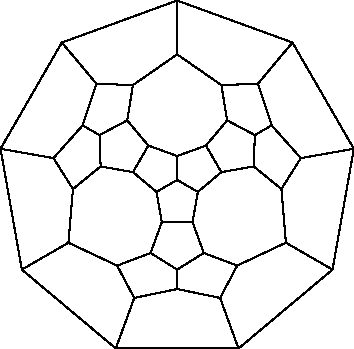
\includegraphics[width=0.8\textwidth]{./Asymptote_Figs/Grinberg3.pdf}
	\end{minipage}
	\vspace{1cm}
	
	\textbf{Solution}: \\
	
	(a): Define two subgraphs of $G$, $G_A$ and $G_B$, such that $G_A$ includes only the edges of $G$ contained in $A$ (including the Hamiltonian cycle) and $G_B$ includes only the edges contained in $B$. Let $V_A,E_A,F_A$ be the numbers of vertices, edges, and faces of $G_A$. Then 
	\begin{align*}
		\sum_{F\in A} \deg(F) - 2 &= (2E_A - V) - 2(F_A - 1) \\
		&= 2(E_A - F_A) + 2 - V \\
		&= 2(V - 2) + 2 - V\\
		&= V - 2.
	\end{align*}
	Here we are using the fact that each edge of $E_A$ borders exactly two faces of $A$, except for the $V$-many edges on the boundary of $A$, which border exactly 1. We also use the fact that $V_A = V$, so that $V - E_A + F_A = 2$.
	
	Having shown that this sum is $V-2$, the other sum is also $V-2$ by the same argument, so they are equal.\\
	
	(b): The values of $\deg(F)$ over all faces in this graph are 
	$$
	(5,5,5,5,5,5,5,5,5,5,5,5,5,5,5,5,5,5,5,5,5,8,8,8,9)
	$$
	and the corresponding values of $\deg(F) - 2$ are 
	$$
	(3,3,3,3,3,3,3,3,3,3,3,3,3,3,3,3,3,3,3,3,3,6,6,6,7).
	$$
	If the graph had a Hamiltonian cycle then by (a), we should be able to split the above sequence into two pieces with equal sum. But only one piece has the 7. The piece without the 7 is divisible by 3 and the other is not, which is a contradiction.
	
\end{document}